%% ****** Start of file apstemplate.tex ****** %
%%
%%
%%   This file is part of the APS files in the REVTeX 4 distribution.
%%   Version 4.1r of REVTeX, August 2010
%%
%%
%%   Copyright (c) 2001, 2009, 2010 The American Physical Society.
%%
%%   See the REVTeX 4 README file for restrictions and more information.
%%
%
% This is a template for producing manuscripts for use with REVTEX 4.0
% Copy this file to another name and then work on that file.
% That way, you always have this original template file to use.
%
% Group addresses by affiliation; use superscriptaddress for long
% author lists, or if there are many overlapping affiliations.
% For Phys. Rev. appearance, change preprint to twocolumn.
% Choose pra, prb, prc, prd, pre, prl, prstab, prstper, or rmp for journal
%  Add 'draft' option to mark overfull boxes with black boxes
%  Add 'showpacs' option to make PACS codes appear
%  Add 'showkeys' option to make keywords appear
\documentclass[aps,prl,onecolumn,superscriptaddress,floatfix]{revtex4-1}
%\documentclass[aps,prl,preprint,superscriptaddress]{revtex4-1}
%\documentclass[aps,prl,reprint,groupedaddress]{revtex4-1}

% You should use BibTeX and apsrev.bst for references
% Choosing a journal automatically selects the correct APS
% BibTeX style file (bst file), so only uncomment the line
% below if necessary.

\usepackage{graphicx}
\usepackage{amsmath}
\usepackage[caption=false]{subfig}
\usepackage{braket}
\usepackage{mathtools}
\usepackage{color}
\graphicspath{{figures/}}
\DeclareMathOperator{\sinc}{sinc}

\begin{document}
\title{Supplemental Material: Amplitude sensing below the zero-point fluctuations with a two-dimensional trapped-ion mechanical oscillator}
\author{K. A. Gilmore}
\email[]{kevin.gilmore@colorado.edu}

\affiliation{National Institute of Standards and Technology, Boulder, Colorado 80305, USA}
\affiliation{JILA and Department of Physics, University of Colorado, Boulder, Colorado, 80309, USA}

\author{J. G. Bohnet}
\affiliation{National Institute of Standards and Technology, Boulder, Colorado 80305, USA}

\author{B. C. Sawyer}
\affiliation{Georgia Tech Research Institute, Atlanta, Georgia 30332, USA}

\author{J. W. Britton}
\affiliation{U.S. Army Research Laboratory, Adelphi, Maryland 20783, USA}

\author{J. J. Bollinger}
\email[]{john.bollinger@nist.gov}
\affiliation{National Institute of Standards and Technology, Boulder, Colorado 80305, USA}
\maketitle

\section*{Introduction}
In this supplemental material we provide detailed derivations for a number of theoretical formulas and results of the main text. Specifically, in the first section we derive  the shift in the spin transition frequency due to the coherent amplitude $Z_c$ (Eq. (2) of the main text) from a more basic perspective. We also discuss in detail our modulation scheme. In the second section we derive the lineshape function used in Fig. 2 of the main text. In section 3 we describe the formalism used to determine the optimum signal-to-noise ratio for a measurement of $Z_{c}^2$. We used this optimum signal-to-noise ration to generate the theoretical curve in Fig. 4 of the main text. We also derive the sensitivity limits for phase-incoherent amplitude sensing, where the phase difference between the driven motion and the ODF randomly varies from one realization of the experiment to the next. We show how these limits depend on $\Gamma/(U/\hbar)$, $\delta k$, and $N$. Finally, in section 4 we consider the amplitude sensing limits assuming phase coherence between the spin-dependent force and the driven amplitude. 

\tableofcontents


\section{1. Shift in the spin transition frequency, and the modulation scheme}
Figure 1 shows the Carr-Purcell-Meiboom-Gill (CPMG) sequence used to apply the 1D traveling-wave potential. The interaction of the spin degree of freedom with the 1D traveling-wave potential is given by
\begin{equation}
\hat{H}_{ODF} = U\sum_{i}\sin(\delta k \cdot \hat{z}_{i} - \mu t + \phi)\hat{\sigma}^{z}_{i} = U\sum_{i}\sin(\delta k \cdot \hat{z}_{i})\cos(\mu t - \phi)\hat{\sigma}^{z}_{i} - U\sum_{i}\cos(\delta k \cdot \hat{z}_{i})\sin(\mu t - \phi)\hat{\sigma}^{z}_{i}.
\label{}
\end{equation}
Here we explicitly include a phase $\phi$ for the traveling-wave potential. Without loss of generality, we assumed $\phi = 0$ in the main text. If $\delta k \left< \hat{z}_{i} \right> \ll 1$, then $\left< \cos(\delta k \cdot \hat{z}_{i}) \right> \sim 1$, and the spin precession due to the second term will be bounded by $(U/\hbar)/\mu$.

Typically, $(U/\hbar)/\mu \ll 1$ and thus this term is ignored in most treatments. At low frequencies $\mu \le U/\hbar$ this term could be important, but it may be canceled by advancing the phase of the ODF by $\Delta \phi = \mu(T+t_{\pi})$ at each microwave $\pi-$pulse of the CPMG sequence (see Fig. 1). When $\mu/2\pi = (2n+1)/(2(T+t_{\pi}))$ for some integer $n$, $\Delta\varphi = \pi$ and we recover the quantum lock-in phase advance of \citep{Kotler2011}. This phase advance coherently accumulates spin precession from the first term of Eq. (1) when $\omega/2\pi = (2n+1)/(2(T+t_{\pi}))$. The term that survives our modulation scheme is
\begin{equation}
\hat{H}_{ODF} \simeq U\sum_{i}\sin(\delta k \cdot \hat{z}_{i})\cos(\mu t  - \phi)\hat{\sigma}^{z}_{i}.
\label{}
\end{equation}

We now impose a weak, classically driven COM motion of constant amplitude and phase $\hat{z}_i \rightarrow \hat{z}_i +Z_c\cos(\omega t+\delta)$. This can be thought of as the center of the Penning trap being moved by $\pm Z_c$ at a frequency $\omega$ far from the trap axial frequency $\omega_z$. With $\delta k \, Z_c \ll 1$, we obtain
\begin{equation}
\hat{H}_{ODF} \simeq  U\sum_{i} \left( \delta k \, Z_c \cos(\delta k \cdot \hat{z}_{i})\cos(\omega t + \delta)\cos(\mu t - \phi) + \sin(\delta k \cdot \hat{z}_{i})\cos(\mu t - \phi) \right) \hat{\sigma}^{z}_{i}.
\label{}
\end{equation}
The second term of Eq. (3) is the usual term that gives rise to spin-motion entanglement with the drumhead modes and to effective spin-spin interactions \citep{[][{ (see Supplementary Information).}]Britton2012,[][{ (see Supplementary Information).}]Bohnet2015}. We assume we can neglect this term because we tune $\mu$ far from any drumhead modes.

Deep in the Lamb-Dicke confimenent regime, the $\cos(\delta k \cdot \hat{z}_{i})$ factor in the first term of Eq. (3) equals one. Here we account for the possibility of not being deep in the Lamb-Dicke confinement regime. In this case, and assuming a thermal distribution of modes, $\left< \cos(\delta k \cdot \hat{z}_{i}) \right> = \exp(-\delta k^2 \left< \hat{z}^{2}_{i} \right> / 2) $. This factor is known as the Debye-Waller factor $\rm{\it{DWF}}$. For our conditions all ions have approximately the same Debye-Waller factor, $\rm{\it{DWF}} \approx 0.86$ \citep{Bohnet2015}.

With $\mu \sim \omega$, Eq. (3) can be written as
\begin{equation}
\hat{H}_{ODF} = (U \cdot \delta k \cdot \rm{\it{DWF}}) \,  Z_c\cos((\omega - \mu)t + \delta - \phi) \sum_{i} \frac{\hat{\sigma}^{z}_{i}}{2},
\label{}
\end{equation}
which is Eq. (2) of the main text with $F_0 = U \cdot \delta k \cdot \rm{\it{DWF}}$.

\section{2. Lineshape}
To model the lineshape of the signal, it is necessary to account for the accumulated phase due to the spin-dependent ODF potential without making the simplification that $ \omega = \mu $. This results in a characteristic response function for each sequence. For this Letter, we used an $ m = 8 $ CPMG sequence, as shown in Fig. 1 in the main text and also Fig. 1 of this supplemental material. In the following, we derive the lineshape of this sequence using the modulation discussed in the first section and assuming a delta function source at a frequency $\omega$. This lineshape is used to generate the theory curves of Fig. 2 of the main text. In general, for a CPMG sequence it is necessary to calculate the phase evolution during $2m$ terms of length T, for a total interaction time of $2m$T. For simplicity, we first derive the lineshape for the $ m = 2 $ CPMG sequence (Fig. 1).
\begin{figure}
    \centering
    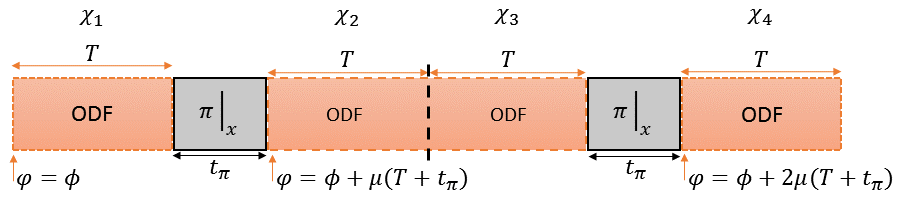
\includegraphics[width=1.0\textwidth]{cpmg_supp}
    \caption{$m = 2$ CPMG sequence with total ODF interaction time $4T$. $\varphi$ is the phase of the ODF beatnote. The $\chi_i$ labels represent the periods over which the accumulated phase is considered in the text.}
    \label{cpmg_sup}
\end{figure}

 For a delta function source $Z_c \cos(\omega t+\delta)$, the spin precession accumulated in a general sequence like that shown in Fig. 1 is

\begin{equation}
\theta(\mu) = F_0 \, Z_c \frac{2 \sin \left( \frac{1}{2}\left(\omega-\mu \right)T \right)}{(\omega-\mu)} \chi(\mu,\omega),
\label{}
\end{equation}
where $\chi(\mu,\omega) = \sum_{i} \chi_i(\mu,\omega)$ is determined by the particular sequence used. In the case of the $ m = 2 $ CPMG sequence, the phase accumulated through four terms corresponding to four separate applications of the ODF (Fig. 1) must be considered:

\begin{equation}
\chi_{1} = \cos \left[  \left( \omega - \mu \right) \frac{T}{2}  + \delta-\phi \right],
\end{equation}

\begin{equation}
\chi_{2} = -\cos \left[  \left( \omega - \mu \right) \left( \frac{3T}{2} + t_{\pi} \right) +\delta-\phi +\mu(T+t_{\pi}) \right],
\end{equation}

\begin{equation}
\chi_{3} = -\cos \left[  \left( \omega - \mu \right) \left( \frac{5T}{2} + t_{\pi} \right) +\delta-\phi +\mu(T+t_{\pi}) \right],
\end{equation}

\begin{equation}
\chi_{4} = \cos \left[  \left( \omega - \mu \right) \left( \frac{7T}{2} + 2t_{\pi} \right) +\delta-\phi +2\mu(T+t_{\pi}) \right].
\end{equation}

Note these terms now include a phase $\phi$ for the ODF interaction, which in the main text we set to zero with no loss of generality. Adding these terms up, pairwise:

\begin{equation}
\chi_{1} + \chi_{2} = 2 \sin \left( \frac{1}{2} \left[  \left( \omega - \mu \right) \left( T + t_{\pi} \right) +\mu(T+t_{\pi}) \right] \right) \sin \left[  \left( \omega - \mu \right) \left( T + \frac{t_{\pi}}{2} \right) +\delta-\phi + \frac{\mu(T+t_{\pi})}{2} \right],
\end{equation}

\begin{equation}
\chi_{3} + \chi_{4} = -2 \sin \left( \frac{1}{2} \left[  \left( \omega - \mu \right) \left( T + t_{\pi} \right) +\mu(T+t_{\pi}) \right] \right) \sin \left[  \left( \omega - \mu \right) \left( 3T + \frac{3t_{\pi}}{2} \right) +\delta-\phi + \frac{3\mu(T+t_{\pi})}{2} \right].
\end{equation}

Summing all four terms yields

\begin{equation}
\chi(\mu,\omega) = \sum_{i} \chi_i(\mu,\omega) = 2 \sin \left( \frac{\omega}{2}\left( T + t_{\pi} \right) \right) \left[ \sin \left( \xi + \delta-\phi \right) - \sin \left( 3\xi + \delta-\phi \right) \right],
\end{equation}
where $\xi = (\omega-\mu)(T+\frac{t_{\pi}}{2})+\frac{\mu(T+t_{\pi})}{2} = \frac{1}{2}\left( \omega (T+t_{\pi}) + T \left( \omega-\mu \right) \right)$.
Then, simplifying:
\begin{equation}
\chi(\mu,\omega) = 2 \sin \left( \frac{\omega}{2}\left( T + t_{\pi} \right) \right) 2 \sin \left(- \xi \right) \cos \left( 2 \xi + \delta-\phi \right).
\end{equation}

Using Eqs. 13 and 5,
\begin{equation}
\theta(\mu) = \rm{\it{DWF}} \cdot U \cdot \delta k \cdot Z_c \cdot T \sinc \left( \frac{T}{2}\left(\omega-\mu \right) \right) 4 \sin \left( \frac{\omega}{2}\left( T + t_{\pi} \right) \right) \sin \left( \xi \right) \cos \left( 2 \xi + \delta-\phi \right).
\end{equation}

Since $4T = \tau$ for the $m = 2$ CPMG, then

\begin{equation}
\theta(\mu) = \theta_{max} \sinc \left( \frac{T}{2}\left(\omega-\mu \right) \right) \sin \left( \frac{\omega}{2}\left( T + t_{\pi} \right) \right) \sin \left( \xi \right) \cos \left( 2 \xi + \delta-\phi \right),
\end{equation}
where $\theta_{max} \equiv (F_{0}/\hbar)\, Z_c \, \tau$, the maximum precession angle on resonance as defined in the main text. Then, $\theta_{max}(\mu)$, defined as $\theta(\mu) = \theta_{max}(\mu) \cos \left( 2 \xi + \delta-\phi \right)$, is the $\mu$-dependent generalization of $\theta_{max}$. From Eq. 15, this is
\begin{equation}
\theta_{max}(\mu) = \theta_{max} \sinc \left( \frac{T}{2}\left(\omega-\mu \right) \right) \sin \left( \frac{\omega}{2}\left( T + t_{\pi} \right) \right) \sin \left( \xi \right).
\end{equation}
For the $m = 8$ CPMG sequence the same procedure is used, but now with 16 periods of accumulated phase. We obtain

\begin{widetext}
\begin{equation}
\theta_{max}(\mu) = \theta_{max}  \sinc\left( \frac{T}{2} \left( \omega-\mu \right) \right) \sin\left( \frac{\omega}{2} \left( T+t_{\pi} \right) \right) \sin(\xi)\cos(2 \xi)\cos(4 \xi).
\end{equation}
\end{widetext} 

As shown in the main text, the expression for population in $\ket{\uparrow}$ - now with a dependence on the ODF difference frequency $\mu$ - is

\begin{equation}
\left< P_{\uparrow} \right> = \frac{1}{2} \left[ 1-e^{-\Gamma \tau}J_0(\theta_{max}(\mu)) \right].
\label{Bessel}
\end{equation}
Equations (17) and (18) are used to obtain the theoretical line shapes of Fig. (2) of the main text.
\section{3. Phase-incoherent sensing limits}

Here we derive Eq. (5) from the main text and provide additional mathematical background for the phase-incoherent experimental protocol, wherein the phase of the measured quadrature varies randomly from one realization of the experiment to the next. Following earlier discussions, the probability of measuring $\left|\uparrow\right\rangle $
at the end of the Ramsey sequence is 
\begin{equation}
\left\langle P_{\uparrow}\right\rangle =\frac{1}{2}\left[1-e^{-\Gamma\tau}J_{0}\left(\theta_{max}\right)\right]\:,\label{eq:P_up formula}
\end{equation}
where $\left\langle \:\right\rangle $ denotes an average over many
experimental trials and therefore over the random phase between the
1D traveling-wave potential and the classically driven COM motion, and
\begin{equation}
\theta_{max}=(F_{0}/\hbar) \cdot Z_{c}\cdot\tau\:.\label{eq:theta_max formula}
\end{equation}
Defining $G\left(\theta_{max}^{2}\right)\equiv\left(1-J_{0}\left(\theta_{max}\right)\right)/2$
and denoting $\left\langle P_{\uparrow}\right\rangle _{bck}=\left[1-e^{-\Gamma\tau}\right]/2$
as the probability of measuring $\left|\uparrow\right\rangle $ at
the end of the sequence in the absence of a classically driven motion,
$\theta_{max}^{2}$ can be determined from a measurement of the difference
$\left\langle P_{\uparrow}\right\rangle -\left\langle P_{\uparrow}\right\rangle _{bck}$
through
\begin{equation}
G\left(\theta_{max}^{2}\right)=e^{\Gamma\tau}\left(\left\langle P_{\uparrow}\right\rangle -\left\langle P_{\uparrow}\right\rangle _{bck}\right)\:.\label{eq:P_up difference}
\end{equation}
The standard deviation $\delta\theta_{max}^{2}$ in estimating $\theta_{max}^{2}$
is determined from the standard deviation $\sigma\left(P_{\uparrow} - P_{\uparrow, bck}\right)$
of the $\left\langle P_{\uparrow}\right\rangle -\left\langle P_{\uparrow}\right\rangle _{bck}$
difference measurements through
\begin{equation}
\delta\theta_{max}^{2}=\frac{e^{\Gamma\tau}\sigma\left(\left\langle P_{\uparrow}\right\rangle -\left\langle P_{\uparrow}\right\rangle _{bck}\right)}{\frac{\mathrm{d}G\left(\theta_{max}^{2}\right)}{d\theta_{max}^{2}}}\:.\label{eq:delta theta^2}
\end{equation}
The signal-to-noise ratio of a measurement of $\theta_{max}^{2}$
(and therefore $Z_{c}^{2}$) is $\theta_{max}^{2}/\delta\theta_{max}^{2} = Z_{c}^{2}/\delta Z_{c}^{2}$.
In general this signal-to-noise ratio depends on $\theta_{max}^{2}$
and the experimental parameters $U\cdot\tau$, $\Gamma\cdot\tau$, $\delta k$, and $N$.

We use Eq. (\ref{eq:delta theta^2}) to theoretically estimate $Z_{c}^{2}/\delta Z_{c}^{2}$
and the amplitude sensing limits. We assume the only sources of noise
are projection noise in the measurement of the spin state and fluctuations
in $P_{\uparrow}$ due to the random variation in the relative phase
of the 1D traveling-wave potential and the driven COM motion. Experimentally this is obtained by collecting ~10 photons for each $\ket{\uparrow}$ state, so photon counting shot noise can be neglected \citep{[][{ (see Supplementary Information).}]Bohnet2015}. In this case
$\sigma\left( P_{\uparrow}-P_{\uparrow,bck}\right)=\sqrt{\sigma_{P_{\uparrow}}^2+\sigma_{P_{\uparrow, bck}}^2}$
where the relevant variances are
\begin{equation}
\sigma_{P_{\uparrow, bck}}^2=\frac{1}{N}\left\langle P_{\uparrow}\right\rangle _{bck}\left(1-\left\langle P_{\uparrow}\right\rangle _{bck}\right)=\frac{1}{4N}\left(1-e^{-2\Gamma\tau}\right)\label{eq:Pbck noise}
\end{equation}
and
\begin{equation}
\sigma_{P_{\uparrow}}^2=\sigma_{\delta}^{2}+\frac{1}{N}\left\langle P_{\uparrow}\right\rangle \left(1-\left\langle P_{\uparrow}\right\rangle \right)\:.\label{eq:Pup noise}
\end{equation}
Here $N$ is the number of spins. Equation (\ref{eq:Pbck noise})
and the second term in Eq. (\ref{eq:Pup noise}) are projection noise.
The variance 
\begin{equation}
\sigma_{\delta}^{2}=\left\langle P_{\uparrow}^{2}-\left\langle P_{\uparrow}\right\rangle ^{2}\right\rangle =\frac{e^{-2\Gamma\tau}}{8}\left(1+J_{0}\left(2\theta_{max}\right)-2J_{0}\left(\theta_{max}\right)^{2}\right)\label{eq:phase fluctuation variance}
\end{equation}
is due to the random variation in the relative phase of the 1D traveling-wave and the driven COM motion. For our set-up, $\rm{\it{DWF}}=\exp(-\delta k^2 \left< \hat{z}^{2}_{i} \right> / 2) =0.86$ and
$\delta k=2\pi/\left(900\:\mathrm{nm}\right)$ are fixed, the
decoherence $\Gamma$ is a function of $U$, $\Gamma=\xi\left(U/\hbar\right)$
where $\xi=1.156\times10^{-3}$, and $F_{0} = \rm{\it{DWF}} \cdot U \cdot \delta k$. For a given $Z_{c}$ we use Eqs.
(\ref{eq:theta_max formula}) and (\ref{eq:delta theta^2})-(\ref{eq:phase fluctuation variance})
to find the optimum $Z_{c}^{2}/\delta Z_{c}^{2}$ as
a function of $\left(U\tau\right)/\hbar$. This optimum value is the red dashed
theoretical curve plotted in Fig. 4 of
the main text.

The signal-to-noise $Z_{c}^{2}/\delta Z_{c}^{2}$ is optimized
for relatively small values of $\theta_{max}^{2}$ where $G\left(\theta_{max}^{2}\right)\approx\theta_{max}^{2}/8$
is a good approximation. This leads to some simplifications for Eqs.
(\ref{eq:P_up difference}) and (\ref{eq:delta theta^2}),
\begin{equation}
\theta_{max}^{2}\approx8e^{\Gamma\tau}\left(\left\langle P_{\uparrow}\right\rangle -\left\langle P_{\uparrow}\right\rangle _{bck}\right)\label{eq:theta_max^sq}
\end{equation}
and
\begin{equation}
\delta\theta_{max}^{2}\approx8e^{\Gamma\tau}\sigma\left(P_{\uparrow} - P_{\uparrow,bck}\right)\:,\label{eq:delta theta_max^2}
\end{equation}
and to the following estimate for the signal-to-noise ratio of a single
measurement,
\begin{equation}
\frac{\theta_{max}^{2}}{\delta\theta_{max}^{2}} = \frac{Z_{c}^{2}}{\delta Z_{c}^{2}} \approx\frac{\left\langle P_{\uparrow}\right\rangle -\left\langle P_{\uparrow}\right\rangle _{bck}}{\sigma\left(P_{\uparrow} - P_{\uparrow,bck}\right)}\:.\label{eq:S/N limits}
\end{equation}
Figure (4) of the main text uses Eq. (\ref{eq:S/N limits}),
along with repeated measurements of $P_{\uparrow} - P_{\uparrow,bck}$,
to experimentally determine the signal-to-noise ratio as a function
of the imposed amplitude $Z_{c}$ of the COM motion.

Finally we use Eqs. (\ref{eq:theta_max formula}) and (\ref{eq:delta theta^2})-(\ref{eq:phase fluctuation variance})
to calculate the sensing limits for very small $Z_{c}$. For small
$Z_{c}$ the variance $\sigma_{\delta}^{2}$ can be neglected compared
to projection noise and $\sigma_{P_{\uparrow}}^2\approx\sigma_{P_{\uparrow, bck}}^2$.
In this case we obtain the following expression for the signal-to-noise
ratio,
\begin{equation}
\frac{Z_{c}^{2}}{\delta Z_{c}^{2}}=\frac{\sqrt{N}}{4\sqrt{2}}\frac{\rm{\it{DWF}}^{2}\cdot\left(\delta k\,Z_{c}\right)^{2}\left(U\tau/\hbar\right)^{2}}{\sqrt{e^{2\xi U\tau/\hbar}-1}}\:.\label{eq:limiting sensitivity}
\end{equation}
Equation (\ref{eq:limiting sensitivity}) is maximized for $\xi U\tau\approx1.9603$, resulting in 

\begin{equation}
\left.\frac{Z_{c}^{2}}{\delta Z_{c}^{2}}\right|_{\mathrm{limiting}}\approx 0.097 \frac{\sqrt{N}(\rm{\it{DWF}})^2 (\delta k)^2}{\xi^2} Z_c^2\:,
\end{equation}
which is Eq. (5) of the main text.
With $\rm{\it{DWF}}=0.86$, $\delta k=2\pi/\left(900\:\mathrm{nm}\right)$,
$\xi=1.156\times10^{-3}$, and $N=85$,
\begin{equation}
\left.\frac{Z_{c}^{2}}{\delta Z_{c}^{2}}\right|_{optimum}=\left[\frac{Z_{c}}{0.2\:\mathrm{nm}}\right]^{2}\:.\label{eq:26.1 Z_c^2}
\end{equation}
For our set-up and available ODF power, $\xi U\tau/\hbar\approx1.9603$
is realized for $\tau\approx20\:\mathrm{ms}$. A measurement of the
signal and a measurement of the background requires $\sim60\:\mathrm{ms}$, allowing
for $16$ independent measurements of $ P_{\uparrow} - P_{\uparrow,bck}$
in 1 s. The limiting sensitivity is approximately $\left(100\:\mathrm{pm}\right)^{2}$
in a 1 s measurement time, or $\left(100\:\mathrm{pm}\right)^{2}/\sqrt{\mathrm{Hz}}$.
We note that the limiting sensitivity is determined by the ratio $\xi=\Gamma/\left(U/\hbar\right)$.
In particular, the optimum value for Eq. (\ref{eq:limiting sensitivity})
scales as $1/\xi^{2}$.

\section{4. Phase-coherent sensing limits}

With appropriate care the phase of the 1D traveling-wave potential can be stable for long
periods of time with respect to the ion trapping electrodes \citep{Hume2011}, enabling repeated phase-coherent sensing of the same quadrature of the COM motion $Z_{c}\cos(\omega t)$.
In this case the same spin precession $\theta_{max}=\rm{\it{DWF}}\cdot\left(U/\hbar\right)\cdot\delta k\,Z_{c}\cdot\tau$
occurs for each experimental trial, which can be detected to first
order in $\theta_{max}$ (or $Z_{c}$) in a Ramsey sequence with a
$\pi/2$ phase shift between the two $\pi/2$-pulses. Assuming $\sin\left(\theta_{max}\right)\approx\theta_{max}$,
appropriate for small amplitudes $Z_{c}$, the equivalent phase-coherent
sensing expressions for Eqs. (\ref{eq:theta_max^sq}) and (\ref{eq:delta theta_max^2})
are
\begin{equation}
\theta_{max}=2e^{\Gamma\tau}\left(\left\langle P_{\uparrow}\right\rangle -\left\langle P_{\uparrow}\right\rangle _{bck}\right)\label{eq:theta_max coherent}
\end{equation}
and
\begin{equation}
\delta\theta_{max}=2e^{\Gamma\tau}\sigma\left( P_{\uparrow} - P_{\uparrow,bck}\right)\:.\label{eq:delta theta_max coherent}
\end{equation}
For a Ramsey experiment with a $\pi/2$ phase shift, $\left\langle P_{\uparrow}\right\rangle _{bck}=1/2$.
If projection noise is the only source of noise, then for small $Z_{c}$,
$\sigma_{P_{\uparrow}}^2\approx\sigma_{P_{\uparrow, bck}}^2=\frac{1}{N}\cdot\frac{1}{2}\cdot\frac{1}{2}$
and $\sigma\left( P_{\uparrow} - P_{\uparrow,bck} \right)\approx\frac{1}{\sqrt{2N}}$.
The limiting signal-to-noise ratio $\theta_{max}/\delta\theta_{max}$
of a $(P_{\uparrow} - P_{\uparrow,bck})$
measurement is
\begin{equation}
\frac{\theta_{max}}{\delta\theta_{max}}=\frac{Z_{c}}{\delta Z_{c}}=\rm{\it{DWF}}\cdot\left(\delta k\,Z_{c}\right)\cdot\sqrt{\frac{N}{2}}\cdot\frac{\left(U\tau\right)}{\hbar}e^{-\xi U\tau/\hbar}\:.\label{eq:S/N coherent}
\end{equation}
Equation (\ref{eq:S/N coherent}) is maximized for $\xi U\tau/\hbar=1$.
With $\rm{\it{DWF}}=0.86$, $\delta k=2\pi/\left(900\:\mathrm{nm}\right)$,
$\xi=1.156\times10^{-3}$, and $N=100$,
\begin{equation}
\left.\frac{Z_{c}}{\delta Z_{c}}\right|_{optimum}=\frac{Z_{c}}{0.074\:\mathrm{nm}}\:.\label{eq:coherent optimum}
\end{equation}
With $16$ independent measurements of $\left\langle P_{\uparrow}\right\rangle -\left\langle P_{\uparrow}\right\rangle _{bck}$
in 1 s, this corresponds to a limiting sensitivity of $\sim\left(20\:\mathrm{pm}\right)/\sqrt{\mathrm{Hz}}$.
The optimum value for the signal-to-ratio of Eq. (\ref{eq:S/N coherent})
scales as $1/\xi$. By employing spin-squeezed states that
have been demonstrated in this system \citep{Bohnet2015},
$Z_{c}/\delta Z_{c}$ can be improved by another factor
of 2.

Employing this technique to sense motion on resonance with the COM mode
can lead to the detection of very weak forces and electric fields.
The detection of a 20 pm amplitude resulting from a 100 ms coherent
drive on the 1.57 MHz COM mode is
sensitive to a force/ion of $5 \times 10^{-5}\:\mathrm{yN}$, corresponding
to an electric field of $0.35\:\mathrm{nV/m}$.

\bibliographystyle{apsrev4-1}
\bibliography{amplitude_sensing}

\end{document}

